\section{Teórico}

  \definicion{Topic:} QUANTUM ESPRESSO: overview and basic functionalities. The self-consistent cycle. PBC: supercells and k-point sampling.

  \definicion{Speaker:} Ralph GEBAUER (ICTP, Italy).

\subsection{DFT}

  La energía del estado basal de un sistema de $N$ electrones es un funcional de la densidad de carga electrónica $n(\vec{r})$ , \emph{i.e.} $E^{DFT} = E^{DFT} [n(\vec{r})]$ donde
    $$n(\vec{r}) \geq 0 \quad ; \quad \int n(\vec{r}) d\vec{r} = N$$

  Matemáticamente se puede probar que dicho funcional existe, pero su forma exacta es desconocida. En el contexto del formalismo de Kohn-Sham (KS) se tiene
    $$E^{DFT} [n(\vec{r})] = T_s [\left\{ \psi_i \right\}] + E_{ext} [n(\vec{r})] + E_{Har} [n(\vec{r})] + E_{ions} + E_{xc} [n(\vec{r})]$$

  donde los orbitales KS se introducen para aproximar la energía cinética individual ($s = single$) según
    $$T_s [\left\{ \psi_i \right\}] = -\frac{\hbar^2}{2m} \sum_{i=1}^N \int \psi_i^{*} (\vec{r}) \nabla^2 \psi_i (\vec{r}) d\vec{r}$$

  y satisfacen además que
    $$\delta_{ij} = \braket{\psi_i}{\psi_j}\ \ i,j\in[1,N] \quad ; \quad n(\vec{r}) = \sum_{i=1}^N \psi_i^{*} (\vec{r}) \psi_i (\vec{r})$$

  \Obs{Los orbitales KS no son many-body, sino que son monoelectrónicos.}

  Los demás términos energéticos refieren a:
    \begin{itemize}
      \item \textbf{Externos:} atracción Coulómbica entre los electrones y los núcleos.
        $$E_{ext} [n(\vec{r})] = \int n(\vec{r}) V_{ext} (\vec{r}) d\vec{r}$$
      \item \textbf{Hartree:} repulsión Coulómbica interelectrónica.
        $$E_{Har} [n(\vec{r})] = \frac{e^2}{2} \int \frac{n(\vec{r}) n(\vec{r}^{'})}{\norm{\vec{r} - \vec{r}^{'}}} d\vec{r} d\vec{r}^{'}$$
      \item \textbf{Iones:} interacción Coulómbica entre iones (si el sistema en estudio es iónico).
        $$E_{ions} = e^2 \sum_{IJ} \frac{Z_I Z_J}{\norm{\vec{R}_I - \vec{R}_J }}$$
      \item \textbf{Correlación-intercambio:} es la diferencia entre el funcional $E^{DFT}$ real (desconocido) y todos los demás términos. Presenta la principal dificultad del método, ya que el funcional $E_{xc} [n(\vec{r})]$ debe ser aproximado de alguna manera.
    \end{itemize}

  En la práctica entonces se minimiza $E^{DFT}$ respecto a $n(\vec{r})$ y, por lo tanto, respecto a los obritales KS. Esto lleva a $N$ ecuaciones KS:
    $$H^{KS} \psi_i (\vec{r}) = \left( -\frac{\hbar^2}{2m} \nabla^2 + V_{ext} (\vec{r}) + V_{Har} (\vec{r}) + V_{xc} (\vec{r}) \right) \psi_i (\vec{r}) = \epsilon_i \psi_i (\vec{r})$$

  donde
    $$V_{xc} (\vec{r}) = \frac{\delta E_{xc}}{\delta n (\vec{r})} \quad ; \quad V_{Har} (\vec{r}) = \frac{\delta E_{Har}}{\delta n (\vec{r})} = e^2 \int \frac{n(\vec{r}^{'})}{\norm{\vec{r} - \vec{r}^{'}}} d\vec{r}^{'}$$

  El problema es que el Hamiltoniano $H^{KS}$ depende de la densidad de carga y, a su vez, la densidad de carga depende de los orbitales KS, los cuales resultan de resolver justamente las ecuaciones de KS: se presenta un problema circular.

\subsection{SCF}

  Para superar el problema circular planteado se recurre a un ciclo autoconsistente (Fig. \ref{fig:SCF}). Al comienzo debemos plantear una densidad de carga inicial, la cual suele ser la superposición de los OA de átomos libres o funciones de onda átomicas aleatorias. A partir de esto podemos construir el Hamiltoniano $H^{KS}$ y resolver las ecuaciones KS. Los orbitales KS resultantes nos permiten definir una nueva densidad de carga.

  Posteriormente, se compara la densidad de carga nueva con la anterior: si la diferencia entre ellas es mayor que el umbral deseado (criterio de convergencia), se define una nueva densidad de carga que resulta de mezclar de alguna manera ambas densidades de carga. La manera más fácil es como está en el esquema, teniendo $0 \leq \alpha \leq 1$. Esta mezcla es esencial para lograr la convergencia ya que agrega cierta fricción al sistema: si simplemente reemplazamos la densidad de carga vieja con la nueva podemos incurrir en oscilaciones infinitas.

  \Obs{En QE el valor de $\alpha$ se declara con $mixing\_beta$.}

  Utilizando la densidad de carga mezclada, se reinicia el ciclo: se construye el Hamiltoniano $H^{KS}$ y se resuelven las ecuaciones KS, obteniendo nuevos orbitales KS que definen una nueva densidad de carga. Cuando la comparación entre densidades de carga sea aceptada por el criterio de convergencia, se considerará que el ciclo autoconsistente ha sido convergente, finalizando el bucle. La densidad de carga asociada al estado basal es la última densidad de carga definida en el proceso.

  \begin{figure}[H]
      \centering
      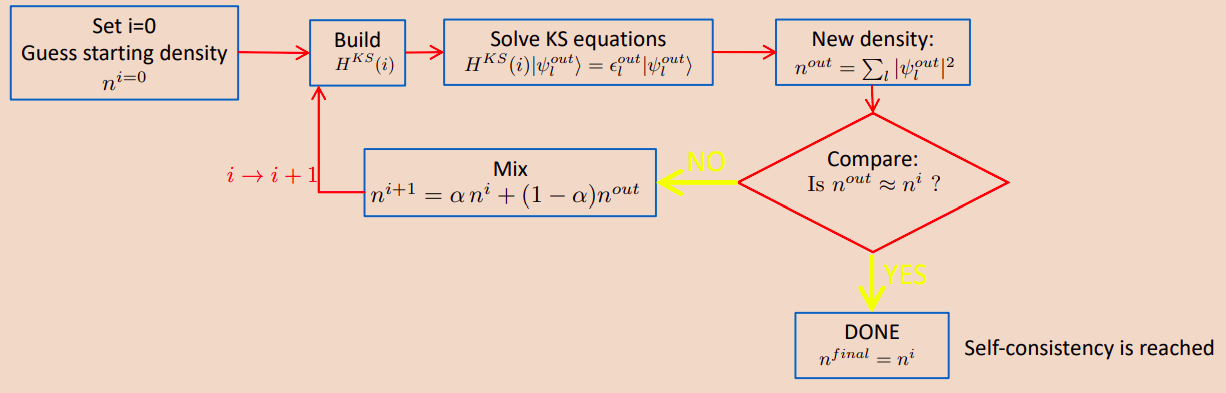
\includegraphics[scale = 0.4]{figs/D1/SCF.png}
      \caption{Esquema del ciclo autoconsistente.}
      \label{fig:SCF}
  \end{figure}

\subsection{PW como base del espacio de Hilbert}

  Dado que la computadora no puede almacenar funciones, sino que simplemente valores, necesitamos una base de funciones $\left\{ b_{\alpha} \right\}_{\alpha=1}^M$ a la cual asociarle dichos valores. A partir de esto definimos una cierta función $f$ como una CL de las funciones de la base según
    $$f (\vec{r}) = \sum_{\alpha = 1}^M c_{\alpha} b_{\alpha} (\vec{r})$$

  donde los coeficientes de la expansión $c_{\alpha}$ son los que se almacenan. El valor de $M$ debe ser lo suficientemente pequeño como para ahorrar memoria, pero lo suficientemente grande como para describir correctamente a $f$.

  El código a utilizar es representado en principio por la base que utiliza. En el caso de QE la base está construida por plane-waves (PW):
    $$b_{\alpha} (\vec{r}) = \frac{1}{\sqrt{V}} \exp{i \vec{G}_{\alpha} \cdot \vec{r}}$$

  \Obs{En QE básicamente todo está definido en términos de combinaciones lineales de senos y cosenos.}

  Los beneficios de utilizar PW como base son:
    \begin{itemize}
      \item Analíticamente simples, pudiendo derivar e integrar fácilmente.
      \item Ortonormales.
      \item No sesgadas: no asume la localización de las cargas ni de los electrones.
      \item Independientes de la posición de los núcleos: la base no va cambiando cuando se mueven los átomos (fuerzas de Pulay).
      \item Fácil control de la convergencia del tamaño de la base.
      \item Aplicación directa de FT, permitiendo aprovechar al máximo las dualidades entre el $R$- y el $G$-espacios.
    \end{itemize}

  Una de las principales desventajas es que el tamaño de la base suele ser mucho mayor que otras bases construidas por funciones localizadas, ya que no poseen información atómica.

\subsection{Periodicidad}

  Dada la naturaleza periódica de las PW, el uso de esta base está íntimamente relacionado con la periodicidad del sistema físico en estudio: son fácilmente aplicables a sistemas periódicos ya que basta definir la red de Bravais y su motivo.

  Si una función es periódica en el $R$-espacio, su FT es no nula únicamente para un conjunto infinito, pero discreto de vectores de onda.

\subsubsection{Caso 1D}

  En el caso de 1 dimensión, se tiene que
    $$\exp{i G_{\alpha}x} \rightarrow G_{\alpha} = n \frac{2\pi}{L} \quad n\in\mathbb{Z}$$

  donde $\sfrac{2\pi}{L}$ es la distancia entre las componentes no nulas de la FT, siendo $L$ el período (tamaño de las unidades que se repiten). A mayor $L$, mayor densidad de puntos no nulos en el $G$-espacio. La longitud de onda asociada a cierto vector de onda $\vec{G}_{\alpha}$ (Fig. \ref{fig:FT_1D}) cumple
    $$\lambda_{\alpha} \propto \frac{1}{\norm{\vec{G}_{\alpha}}}$$

  \begin{figure}[H]
      \centering
      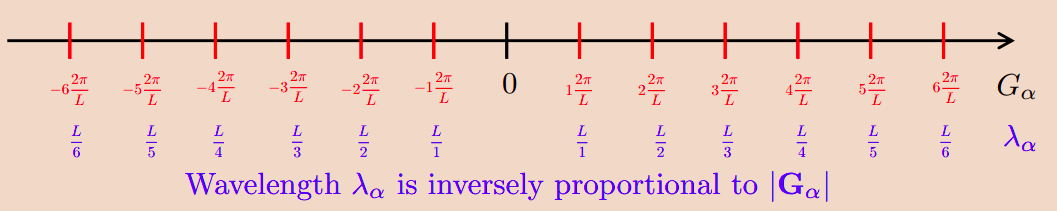
\includegraphics[scale = 0.4]{figs/D1/FT_1D.png}
      \caption{Representación de las infinitas componentes de Fourier en el $G$-espacio, denotando que son discretas. Se tienen además las longitudes de onda asociadas a cada vector de onda con componente no nula.}
      \label{fig:FT_1D}
  \end{figure}

  Aunque hemos logrado una discretización, para poder realizar un cálculo en la práctica necesitamos una cantidad finita de puntos. Para truncar la cantidad de puntos, uno determina una longitud de onda mínima $\lambda_{min}$, la cual sea suficiente para describir las características de interés (Fig. \ref{fig:FT_1D_min}).

  \Obs{Los orbitales y, por lo tanto, la densida de carga no varían en la escala de los núcleos atómicos, sino que varían en la escala de los \si{{\angstrom}}}.

  \begin{figure}[H]
      \centering
      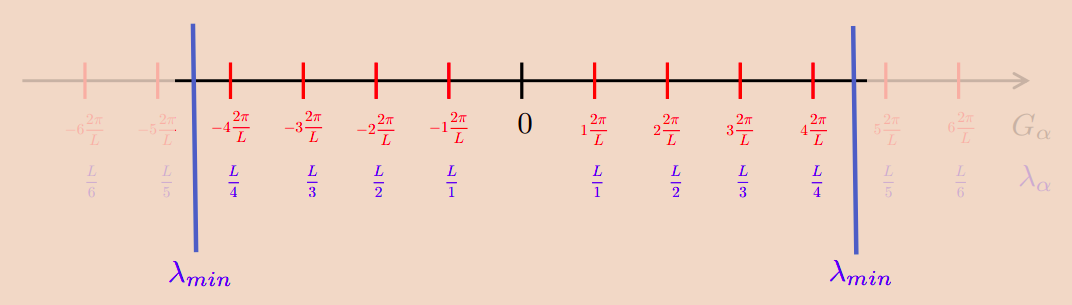
\includegraphics[scale = 0.4]{figs/D1/FT_1D_min.png}
      \caption{Truncamiento de las componentes no nulas en el $G$-espacio a partir de considerar cierto $\lambda_{min}$.}
      \label{fig:FT_1D_min}
  \end{figure}

  En la práctica uno no le dice al programa cuál es $\lambda_{min}$, sino que le indica la norma máxima para el vector de onda.
    $$G_{max} = \frac{2pi}{\lambda_{min}} \quad ; \quad G_{max} \equiv \norm{\vec{G}}_{max}$$

  En QE esto se hace estableciendo el cutoff de la energía cinética:
    $$E_{cut}^{\psi} = \frac{\hbar^2}{2m} G_{max}^2 \quad \equiv ecutwfc\ \ [Ry]$$

  \Obs{Este truncamiento es el que le indica a QE el tamaño de la base de PW. Como la ubicación de los puntos no nulos está directamente ligada al parámetro de red, se puede ver que la modificación de dicho parámetro altera la base de PWs utilizada: a mayor tamaño de red, la grilla de vectores $G$ se hace cada vez más densa y, manteniendo $G_{max}$ fijo, se irán agregando más PW al cálculo de manera discontinua. Esto se observa en una caída brusca en la enerǵia al agrandar el tamaño de la base. Si se presentan estas discontinuidades, hay que definir otras variables en el input: ecfixed, qcutz y q2sigma.}

\subsubsection{Caso 2D}

  Al considerar dos dimensiones, nuevamente tenemos el problema de que aunque son dicretos, tenemos infinitos puntos. En este caso, el truncamiento es una circunferencia (Fig. \ref{fig:FT_2D}). Se tiene
    $$\exp{i \vec{G}_{\alpha} \cdot \vec{r}} \rightarrow \vec{G}_{\alpha} = m \vec{B}_1 + n \vec{B}_2 \quad m,n\in\mathbb{Z}$$
  donde $\vec{B}_{1,2}$ son los vectores recíprocos de la red.

    \begin{figure}[H]
        \centering
        \subfigure[]{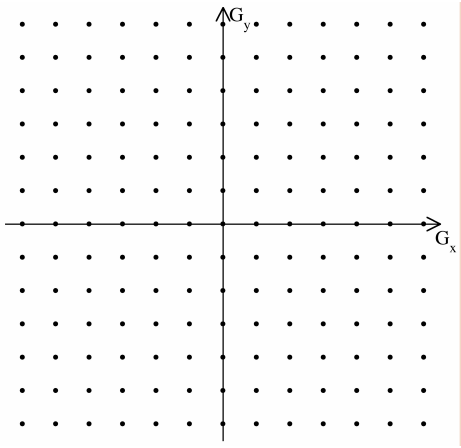
\includegraphics[scale = 0.3]{figs/D1/FT_2D_inf.png}}
        \subfigure[]{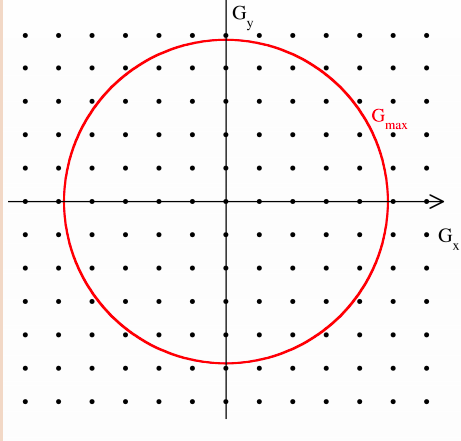
\includegraphics[scale = 0.3]{figs/D1/FT_2D_Gmax.png}}
        \subfigure[]{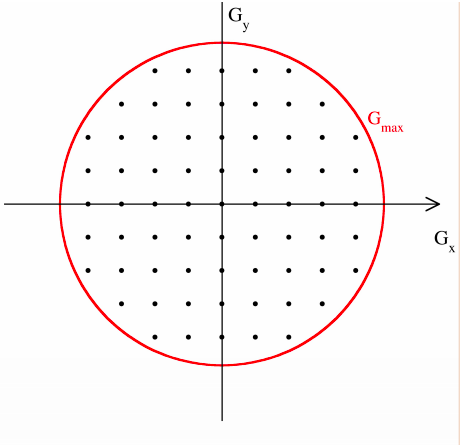
\includegraphics[scale = 0.3]{figs/D1/FT_2D_fin.png}} \\
        \caption{En el caso bidimensional el truncamiento se hace estableciendo una circunferencia de radio $G_{max}$.}
        \label{fig:FT_2D}
    \end{figure}

\subsubsection{Caso 3D}

  Extendiendo a 3 dimensiones:
    $$\exp{i \vec{G}_{\alpha} \cdot \vec{r}} \rightarrow \vec{G}_{\alpha} = m \vec{B}_1 + n \vec{B}_2 + p \vec{B}_3 \quad m,n,p\in\mathbb{Z}$$

  donde $\vec{B}_{1,2,3}$ son los vectores recíprocos de la red. Ahora el truncamiento es una esfera de radio $G_{max}$.

\subsection{Desde los orbitales KS hacia la densidad de carga}

  Considerando todo lo dicho, los orbitales KS expresados como CL de PWs con un cutoff $G_{max}$ son
    $$\psi_i (\vec{r}) = \sum_{\norm{\vec{G}} < G_{max}} c(\vec{G}) \exp{i \vec{G} \cdot \vec{r}}$$

  En el $R$-espacio dijimos que la densidad de carga viene dada por $n(\vec{r}) = \sum_{i=1}^N \psi_i^{*} (\vec{r}) \psi_i (\vec{r})$. Al convolucionar obtenemos la densidad de carga en el $G$-espacio:
    $$\tilde{n}(\vec{r}) = \sum_{i=1}^N \sum_{\norm{\vec{G}^{'}} < G_{max}} \tilde{\psi}_i^{*} (\vec{G}^{'}) \tilde{\psi}_i (\vec{G} - \vec{G}^{'})$$

  Al limitar $\norm{\vec{G}^{'}} < G_{max}$ estamos limitando las contribuciones de $\tilde{\psi}_i^{*} (\vec{G}^{'})$. Sin embargo, ahora la norma de $\vec{G}$ puede ser mayor que $G_{max}$ pues incluso cuando $\norm{\vec{G}} = 2 G_{max}$ y $\norm{\vec{G}^{'}} =  G_{max}$, se cumple que $\tilde{\psi}_i (\vec{G} - \vec{G}^{'}) \neq 0$.

  A partir de esto el análisis de Fourier nos dice que como la densidad de carga es un producto de 2 funciones truncadas según $G_{max}$, la densidad tendrá un cutoff mayor. Las componentes de Fourier no nulas estarán limitadas por $2G_{max}$. Este establece que en el cálculo tendremos dos bases: una para los orbitales, limitada por $G_{max}$, y una para la densdiad, conteniendo más puntos en el espacio recíproco ya que está limitada por $2G_{max}$. Esto lleva a la siguiente relación:
    $$E_{cut}^{n} \geq 4 E_{cut}^{\psi} \quad \equiv ecutrho\ \ [Ry]$$

  \Obs{Si no se hace esta distincción, se puede incurrir en aliasing errors. El código automáticamente establece la relación $ecutrho = 4 ecutwf$, teniendo que indicarla de manera explícita cuando necesitamos que un $ecutrho$ mayor.}

\subsection{Teorema de Bloch: primera zona de Brillouin}

  Aunque el sistema sea periódico, los orbitales no son necesariamente periódicos. En un sistema periódico, los orbitales de Bloch se relacionan con los orbitales KS según
    $$\psi_{\vec{k},i} (\vec{r}) = \exp{i \vec{k} \cdot \vec{r}} u_{\vec{k},i} (\vec{r})$$

  donde sólo la función $u_{\vec{k},i}$ es periódica ya que $\vec{k}$ no necesariamente es un punto de la grilla en el $G$-espacio, provocando que $\psi_{\vec{k},i}$ no sea periódica. Se tiene que
    $$u_{\vec{k},i} (\vec{r}) = \sum_{\norm{\vec{G}} < G_{max}} c_{\vec{k},i} \exp{i \vec{G} \cdot \vec{r}}$$

  la cual está definida sobre la grilla de $G$-vectores antes definida. Luego
    $$\psi_{\vec{k},i} (\vec{r}) = \sum_{\norm{\vec{G}} < G_{max}} c_{\vec{k},i} \exp{i \left(\vec{k} + \vec{G}\right) \cdot \vec{r}} $$

  obteniéndose una grilla corrida de $(k+G)$-vectores. A pesar del corrimiento, el cutoff no se ve alterado (Fig. \ref{fig:kg}).

    \begin{figure}[H]
        \centering
        \subfigure[]{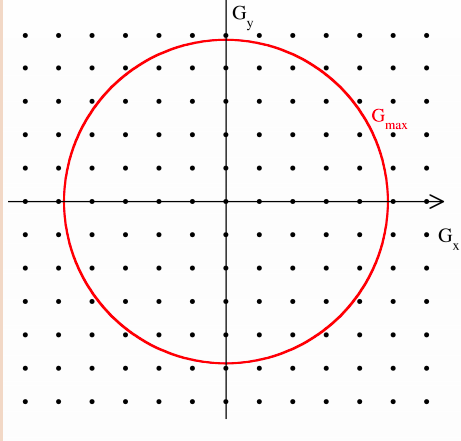
\includegraphics[scale = 0.3]{figs/D1/FT_2D_Gmax.png}}
        \subfigure[]{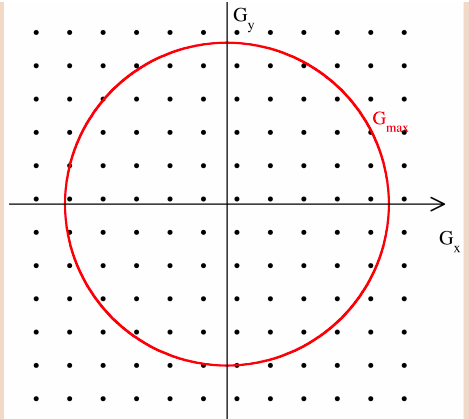
\includegraphics[scale = 0.3]{figs/D1/kg_1.png}} \\
        \subfigure[]{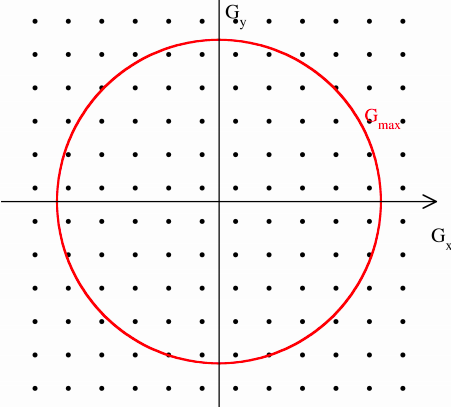
\includegraphics[scale = 0.3]{figs/D1/kg_2.png}}
        \subfigure[]{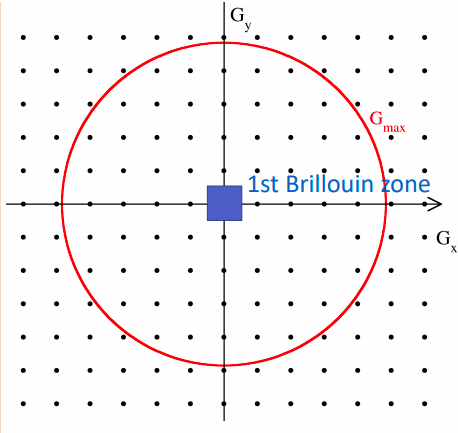
\includegraphics[scale = 0.3]{figs/D1/1BZ.png}} \\
        \caption{Grilla de $G$-vectores (a) comparada con dos posibles grilals de $(k+G)$-vectores, según dos posibles valores para $k$ (b y c). Se esquematiza además la 1BZ (d).}
        \label{fig:kg}
    \end{figure}

  Si al vector $\vec{k}$ se le suma un vector recíproco el resultado es indistinguible dada la periodicidad del sistema en el espacio recíproco. Esto lleva a que sólo sea necesario considerar la primera zona de Brillouin (1BZ): cualquier punto por fuera de la 1BZ será mapeado por el corrimiento a algún punto dentro de la 1BZ dada la periodicida. De este modo, aunque en un sistema periódico debemos sumar sobre todos los posibles valores de $k$-vectores, los únicos relevantes son aquellos que yacen dentro de la 1BZ. Luego, es importante hacer un buen muestreo de 1BZ.

  Supongamos que tenemos en 2 dimensiones una 1BZ rectangular cuyos vectores recíprocos son $\vec{B}_1$ y $\vec{B}_2$. Deseamos muestrear la 1BZ con una grilla de $k$-puntos de 4x4. Si la grilla es corrida en la mitad de la distancia que separa dos $k$-puntos consecutivos (Fig. \ref{fig:shift}), la convergencia será más rápida: dada la simetría que se genera, disminuyen la cantidad de cálculos que deben ser llevados a cabo. Sin embargo, en el caso no corrido, siempre tendremos presente el punto $k=0$ sin importar la simetría del sistema, pero se pierde al hacer el corrimiento.

  \Obs{En QE el corrimiento se hace cambiando los 0 por 1 en la carta de K\_POINTS automatic. Los cálculos con corrimiento no son comparables entre supercells (sistemas no 3D-periódicos) de tamaños diferentes por la pérdida de $k=0$. Generalmente conviene usar cuando tengo un sistema periódico que quiero que converja rápido.}

  \begin{figure}[H]
      \centering
      \subfigure[]{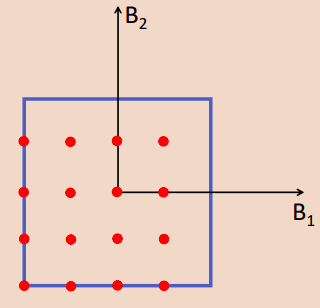
\includegraphics[scale = 0.4]{figs/D1/noshift.png}}
      \subfigure[]{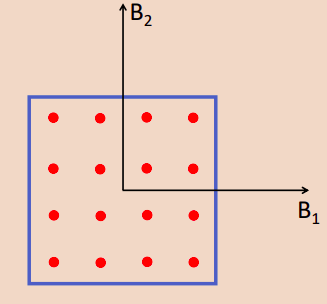
\includegraphics[scale = 0.4]{figs/D1/shift.png}} \\
      \caption{Muestreo de una 1BZ en 2 dimensiones con una grilla 4x4: original (a) y corrida (b).}
      \label{fig:shift}
  \end{figure}

\subsection{Sistemas no 3D-periódicos}

  Cuando se tiene un sistema que no es 3D-periódico, la solución es utilizar una supercelda: se agrega suficiente vacío en la celda como para que el sistema no vea a sus imágenes. Suficiente quiere decir tal que las interacciones entre ellas sean despreciables. De este modo evitamos interacciones espúreas.

  El problema de esto es cuando el sistema en estudio es cargado o dipolar: debido a la lentitud con la que decaen estas interacciones, deberíamos usar superceldas enormes. Para superar este problema existen dos soluciones:
    \begin{enumerate}
      \item Usar la variable assume\_isolated en el input, la cual es muy útil en sistemas 0D (moléculas, clusters, etcétera).
      \item Introducir una caoa dipolar en el vacío entre dos slabs consecutivos, utilizando la variable dipfield en el input.
    \end{enumerate}

\subsection{Pseudopotenciales}

  Si se considera la contribución radial de una función de onda para un cierto núcleo, se observa que en las cercanías del núcleo se presentan oscilaciones muy rápidas. Si quisiéramos muestrear esta primera región, necesitaríamos un $\lambda_{min}$ muy pequeño, lo que implicaría un cutoff muy grande para la energía cinética y, por lo tanto, una base de PWs mucho mayor (cálculo extremadamente caro). Sin embargo, en esta distancia no está la química pues es el core: todo ocurre a distancias mayores respecto al núcleo, donde la función ya es mucho más suave.

  El pseudopotencial da lugar a una pseudofunción de onda que tiene exactamente el mismo comportamiento que la función de onda original para todo radio mayor a cierto radio de corte ($r_{cut}$), pero que por debajo de dicho valor tiende suavemente a cero (Fig. \ref{fig:pseudo}). Esta pseudofunción de onda queda descripto por un $\lambda_{min}$ mayor, requieriéndose una base más pequeña, dando lugar a un cálculo más barato.

  \Obs{Los pseudopote afectan $V_{ext}$ en la ecuación KS.}

  \begin{figure}[H]
      \centering
      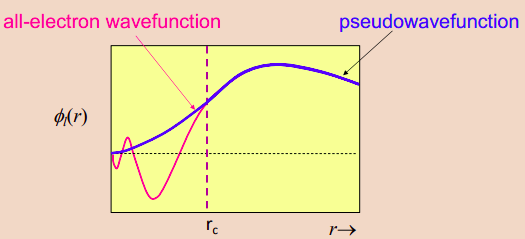
\includegraphics[scale = 0.6]{figs/D1/pseudo.png}
      \caption{Comparación de la función de onda original (all-electron) y la función de onda generada a partir del pseudopotencial.}
      \label{fig:pseudo}
  \end{figure}

  La condición necesaria para que el pseudopotencial sea transferible es que sea norm-conserving, \emph{i.e.} que la norma de ambas funciones sea la misma para valores por debajos del $r_{cut}$. De lo contrario, el átomo no tendrá las propieades de dispersión adecuadas.
    $$\int_0^{r_{cut}}\phi_{AE}^{*} (r) \phi_{AE} (r) dr = \int_0^{r_{cut}}\phi_{PS}^{*} (r) \phi_{PS} (r) dr$$

  \Obs{En la página materialsclouding.org/discover/sssp se tienen pseudopotenciales confiables.}

  Las características de un pseudopotencial son (Fig. \ref{fig:pseudoo}):
    \begin{itemize}
      \item Más débiles que un potencial coulómbico.
      \item No presentan singularidades en $r=0$.
      \item Iguales para $r$ grandes, pero dependientes del momento angular $l$ para $r$ pequeños.
    \end{itemize}

    \begin{figure}[H]
        \centering
        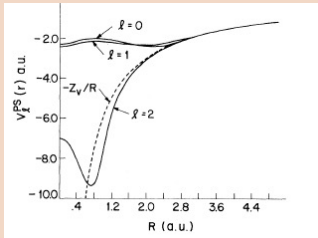
\includegraphics[scale = 0.6]{figs/D1/pseudoo.png}
        \caption{Comparación de un pseudopotencial con el potencial Coulómbico.}
        \label{fig:pseudoo}
    \end{figure}

  En QE los pseudopotenciales (PP) son provistos por el usuario en forma de archivos, que contienen la descripción del PP en una grilla radial. Los PP son específicos para cada elemento químico. Además, son dependientes del funcional utilizado: el código detecta automáticamente cuál fue el funcional utilizado y lo utilizará para resolver las ecuaciones KS. En este sentido, es conveniente que todos los PP que se usan en una misma corrida hayan sido creados considerando el mismo funcional.

\subsubsection{Problemas con la conservación de la norma}

  Existen ciertos elementos para los cuales la condición de conservación de la norma termina siendo un problema: se dan cutoffs mayores de lo que uno querría. Esto ocurre especialmente cuando la función de onda no tiene nodos.

  En estos casos uno puede remover la condición de conservación de norma. Sin embargo, para que los resultados sean confiables, debemos recurrir a una expresión más complicada para la densidad de carga electrónicas
    $$n (\vec{r}) = \sum_{i=1}^N \psi_i^{*} (\vec{r}) \psi_i (\vec{r}) + n^{aug} (\vec{r})$$

  donde el término $n^{aug}$ es la augmentation charge density, la cual está localizada en torno al núcleo y da cuenta de la norma que se estaba perdiendo, expresada en términos de proyectores.

  Este es el caso de los ultrasoft PP (USPP) y los PAW PP. Tenemos entonces que, a pesar de que la norma no se conserva mediante la misma condición de antes, logramos alcanzar la misma norma al sumarle este nuevo término. Las consecuencia de esto es que necesitamos cutoff mayores ($E_{cut}^{n} > 4 E_{cut}^{\psi}$) y, por lo tanto, debemos darle a QE ambos valores necesariamente: tanto ecutwfc como ecutrho. Esto lleva a que haya que chequear la convergencia de ambos parámetros.

\section{Q\&A}

  \definicion{What is the reason for the weight $\alpha$ for the density? Why not just take n\_out in the scf cycle?}

  The mixing parameter (not weight!) $\alpha$ is important for the SCF cycle to converge. If you simply take n\_out, then is is very likely that you only oscillate between various densities. The mixing (which is in reallity more sophisticated that what I have shown in the slides) akts like a friction term. You add only a (normally small) piece of the new density, guaranteeing that step by step you approach the self-consistent solution

  \definicion{what is the convergency criterion? what does the total scf accuracy in every iteration measure? the difference between the current and previous total energy?}

  What the code prints as "scf accuracy" is in fact an energy: it first calculates the difference of the density between "in" and "out", and then estimates an energy by plugging this "$\delta$ rho" into the formula for a Hartree energy. It is in a sense the classical Coulomb interaction energy of the change in density. As "$\delta$\_rho" goes to zero, so does this quantity. Reference: function rho\_ddot in scf\_mod.f90

  \definicion{Do we also check the density separately? How is the convergence checked?}

  The convergence is checked by this quantity (called dr2 in the code). It is not a change in estimated total energy, but a measure of the norm of the change in charge density

  \definicion{US and PAW, what should one chose and when? This ties maybe to a deeper question about how much should the final user care about their choice of PP. To what extent are the PP influencing the results? how realistic is a scenario where I completely have to throw away work because of the wrong choice of pseudopotential? What are the main pitfalls to avoid? Does this availability of multiple pseudos influence reproducibility?}

  From a user's perspective, the choice of either US or PAW is only relevant if you plan to do calculations  where you need to obtain the additional info which PAW can provide you: in PAW you can "reconstruct" the shape of the all-electron wavefunctions close to the nucleus. This info in needed for certain properties, for example if you are interested in NMR chemical shifts. If you are not interested in such (very particular) applications, then you can use US and PAW both in the same way.

  About pseudopotentials in general: in the past, this was a huge issue: many old calculations you find today in the literature are in fact wrong - because of wrong pseudopotentials. Either the potentials were outright wrong, or (more common) people used pseudopotentials where some semi-core electrons were "hidden" in the core, while it would have been important to include them in the (explicitly treated) valence. Today, one knows about the importance of such "semi-core" electrons, and pays more attention.

  As a user, make sure that you do not blindly download PPs from some obscure (and perhaps old) database, where you do not know if the PPs have been checked and controlled carefully. One very exemplary source for PPs (limited to PBE and PBEsol functionals) is this one: https://www.materialscloud.org/discover/sssp/table/efficiency Here, they have made a very thorough and exemplary job of checking everything against all-electron calculations. But also the pslibrary are generally reliable https://www.quantum-espresso.org/pseudopotentials

  As a user, still in every case, check which is the valence configuration for every pseudopotential ("how many electrons are in the valence?") and in case of doubt, compare with another pseudopotential which contains more electrons

  \definicion{I'm confused about the mixing number alpha and beta, since the mixing\_beta is what I include in calculations and I thought this was the mixing parameter responsible of combining old and new densities. Am I mistaken?}

  Sure, this was my fault. What I called $\alpha$ in my talk is called $\beta$ in pwscf ...

  \definicion{In the lecture, there was this dipfield tag recommended for 2D systems. Would that apply to graphene? Could you please comment further on that tag?}

  No need for that in the case of pristine graphene as it does not have the electrostatic dipole moment. The dipole layer correction should be applied only in cases when you have a 2D material (which lies in x0y plane) that is an insulator and has considerable dipole moment pointed in the z-direction. In such cases the electrostatic potential is not the same on both sides of 2D material, thus the dipole layer correction should be applied. Usually you apply it when you want to calculate the work function.

  \definicion{If I doing scf calculation i don’t know how me bands looks like. How do I know that I have insulated system or the system have dipole moment?}

  Best way: plot density of states with dos.x after you do scf and nscf. I recommend this.

  Quickest way: in the \&CONTROL flag of the pw.graphene.scf.in set the verbosity='high' and do the calculation with smearing turned on. Then in the output file you will get the occupation numbers for all the k-points. If some of them are fractional numbers then you got a metal.

  NB. In case of graphene, when you do not have included the special point K in the k-point grid and you have very small smearing you will falsely get a narrow gap semiconductor (the gap is decreasing with the number of k-points but will never go away unless you include point K or increase the smearing).

  \definicion{When I have to use vdw corretion (vdw\_corr) in scf calculation?}

  You use vdw\_corr when you have two subsystems A and B that are interacting very weakly, usually by means of dipol-(induced) dipol interaction. Those kind of interactions are called van der Waals interactions. For instance, when you adsorb graphene on top of Ni(111) and you want to calculate adsorption energy with PBE functional, if you do not put vdw\_corr you won't be able to obtain the adsorption energy, it will be basically zero.

  Or even simpler example - you have bilayer graphene and you use PBE functional to obtain the interaction (adhesion) energy between two sheets. If you plot E\_adh vs distance you will see that there is no minimum. On the other hand, if you put vdw\_corr you will clearly see the minimum at some distance between 2 and 3 angstroms

  \definicion{In the second example from today, why do the number of k-points change from the scf to the nscf calculation? (from 9 9 1 to 12 12 1)}

  because we compute the DOS with the tethraedra method that need a denser mesh

  it is not so crucial as in the scf case, in particulare for DOS and pDOS is more about about the quality of the plot, but in principle yes one should check whether denser mesh change the result significantly

  \definicion{What are the main reasons for choosing one Pseudopotential over another?}

  1. accuracy ; 2. economy; 3. a tradeoff between 1 and 2

  \definicion{I have a qustion regarding k-grid. As this parameter is a consequence of periodicity - what do I do with amorphous cell? Gamma-only because of no long-range order or test k-grids?}

  A test is necessary... Even if you think that the system is “aperiodic”, for the electrons it is not. If you have a small cell, your electrons will “see” the periodicity, and thus there is band dispersion, and thus sampling of the Brillouin zone is needed. If you have a large cell, the periodicity through the cell is no longer “seen” by the electrons, and Gamma-only is sufficient. Your system is probably between these two extrema, very small and extensively large, and thus, depending on the size and type of electronic structure, you might be forced to test for the convergence indeed.

  PS: for a disordered system, you can think of k-point sampling as of a sampling over boundary conditions for the wavefunctions. At k=0, wavefunctions are periodic over the simulation cell. At zone border, they are antiperiodic, etc. As the choice of boundary conditions is to a large extent a matter of convention, it makes sense to sample different choices for them. For large enough systems, calculated properties are independent of the boundary conditions, and sampling just the Gamma point would do.

  \definicion{how do I choose an appropriate mixing\_beta parameter for each system?}

  You start from the default value. Which is 0.7. In most cases this is ok. If the scf cycle does not converge, then use a smaller value. Sometimes as small as 0.1 is needed. However, if you encounter serious convergence problems in the scf cycle, then often it helps to introduce some smearing with finite temperature. This avoids that some states discontinuously cross the Fermi level and are therefore occupied/empty in subsequent iterations. Very often, smearing helps more to make your cycle converge than changing mixing\_beta

  \definicion{¿Podría correr con shift en los k-points  para hacer una relajación y, una vez que esté relajado, seguir los cálculos sin el corrimiento?}

\section{Hands-on}

    \definicion{Topic:} How to compile Quantum ESPRESSO. SCF calculations + post-processing – part 1. XCrySDen, PWgui, QE-emacs-modes, and PWTK

    \definicion{Speaker:}	Pietro DELUGAS (SISSA, Italy).

\subsection{Benzene}

\subsubsection{Objetivo} Aprender a calcular y plotear orbitales moleculares en benceno.

\subsubsection{Pasos}
    \begin{enumerate}
      \item Hacer un cálculo SCF (pw.x) para determinar los estados KS.
        \begin{verbatim}
          pw.x < pw.benzene.scf.in > pw.benzene.scf.out
        \end{verbatim}
      \item Calcular todos los MO de valencia y el LUMO (pp.x) según $sign(\psi (\vec{r})) \norm{\psi (\vec{r})}^2$. Los resultados se escriben en un archivo psi2.benzene\_K001\_B0*.xsf.
        \begin{verbatim}
          pp.x < pp.benzene.psi2.in > pp.benzene.psi2.out
        \end{verbatim}
      \item Graficar uno de los archivos XSF generados con xcrysden. Por ejemplo
        \begin{verbatim}
          xcrysden --xsf psi2.benzene_K001_B006.xsf
        \end{verbatim}

            Luego, mejorar la calidad de la gráfica y guardar el estado (File-->Save Current State). Supongamos que el estado fue guardado como MO-state.xcrysden, luego el estado puede levantarse con otro orbital haciendo
        \begin{verbatim}
          xcrysden --xsf psi2.benzene_K001_B005.xsf --script MO-state.xcrysden
        \end{verbatim}
      \item Para graficar todos los MO ejecutar en la terminal
        \begin{verbatim}
          ./plot-psi2.sh
        \end{verbatim}
    \end{enumerate}

\subsubsection{Resultados}

  En los inputs, QE toma como comentarios a aquellas líneas que comienzan con ! o con \#. Si no se escriben los valores para $pseudo\_dir$ y $outdir$, pw.x va a recurrir a los variables de ambiente: ESPRESSO\_PSEUDO y ESPRESSO\_TMPDIR, respectivamente (esto lo definimos en el .bashrc).

  En la carpeta de archivos temporales se genera, por cada prefix, una carpeta (prefix.save/) y un archivo XML (prefix.xml): la carpeta contiene binarios para hacer procesamientos posteriores, mientras que en el xml se tiene información general acerca de la corrida.

  Para los cálculos se utilizaron USPP con PBE como funcional:
    \begin{itemize}
      \item C.pbe-rrkjus.UPF
      \item H.pbe-rrkjus.UPF
    \end{itemize}

  Se puede usar emcas para que reconozca las variables relevantes del QE, sino se pueden crear unos archivos que permiten que vim las detecte (https://github.com/leseixas/quantum\_espresso-vim).

  Se conocen como namelists a aquellos bloques que comienzan con \&, mientras que los demás bloques se denominan cards.

  Para correr sobre M procesadores (teniendo mpi):
    \begin{verbatim}
      mpirun -np M pw.x -i input\_file.in > output\_file.out
    \end{verbatim}

  Si escribimos
    \begin{verbatim}
      mpirun -np M pw.x -i input\_file.in | tee output\_file.out
    \end{verbatim}

  nos irá mostrando el cálculo en pantalla además de guardarl en el archivo de destino.

  En pp.x dentro del namelist \&INPUTPP las variabes kband(1) y kband(2) le indican desde y hasta qué orbital queremos calcular, respectivamente. En este caso queremos los 16 orbitales. Además lsign le pide que conserve el signo de la función cuando es .true.

  Luego en la namelist \&PLOT tenemos:
    \begin{itemize}
      \item \textbf{iflag:} como es 3 le estamos pidiendo que grafique en 3 dimensiones.
      \item \textbf{nfile:} le indica que sólo debe considerar un archivo.
      \item \textbf{weight(1):} en este caso sólo hay un archivo (nfile=1) y por eso se le pone peso 1. Sin embargo, podría tener más de un archivo que considerar y con esta variable puedeo ponderar dicha consideración.
    \end{itemize}

  Al correr pp.x se van a generar 2 arhivos por orbital: uno propio de QE y otra para que pueda ser levantado por xcrysden.

  Para que xcrysden considere la información del orbital, debemos ir a $Tools > Datagrid$ y seleccionar lo que deseamos graficar (en este caso sólo habrá una opción disponible ya marcada dentro de la gráfica de árbol). El mutiply factor es la densidad de carga dividido el volumen de la celda. Al estar usando una molécula asilada, la celda es mucho mayor que la densidad de carga. Luego debemos usar un valor grande: usaremos 100.

  Al dar $ok$ se abre un nuevo menú. Lo que nos interesa es ingresar un isovalor para la densidad de carga electrónica (cuadrado rosa vacío). Este valor debe encontrarse entre los extremos que están por encima de este cuadrado y en grisesito. Esto permitirá que se genere una isosuperficie. Conviene tildar $Render +/- isovalue$ para detectar las zonas con densidad de carga de diferente signo. Al poner $Submit$ vemos que sobre la molécula se grafican los orbitales.

  \Obs{No hay una regla para elegir el isovalor. Debe ser uno tal que permita observar claramente todas las características de lo que queremos mostrar. Si vamos a comparar entre varias isosuperficies, hay que chequear que todas queden bien presentadas para su análisis utilizando el mismo isovalor. Valores más cercanos a 0 tienden a mostrar isosuperficies más grandes, tendiendo a perderse un poco la cuestión.}

  \begin{figure}[H]
      \centering
      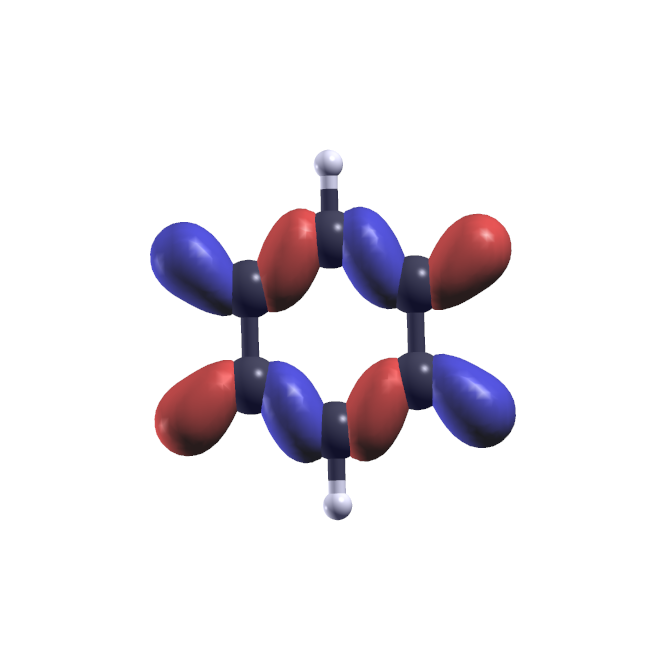
\includegraphics[scale = 0.4]{figs/D1/psi2.benzene.png}
      \caption{Doceavo MO para el benceno.}
  \end{figure}

\subsection{Graphene}

\subsubsection{Objetivo}

  Calcular y plotear DOS y estructura de bandas (spaghetti) de una hoja de grafeno.

\subsubsection{Pasos}

    \begin{enumerate}
      \item Hacer un cálculo SCF (pw.x) para determinar los estados KS.
        \begin{verbatim}
          pw.x < pw.graphene.scf.in > pw.graphene.scf.out
        \end{verbatim}

      \item Plotear DOS:
        \begin{enumerate}
          \item Hacer un cálculo no SCF (pw.x) con una grilla más densa de puntos k (aumenta la \emph{definición} de la DOS).
            \begin{verbatim}
              pw.x < pw.graphene.nscf.in > pw.graphene.nscf.out
            \end{verbatim}
        \item Hacer el cálculo para genera el datafile de la DOS (dos.x). El resultado se escribe en el archivo graphene.dos.
          \begin{verbatim}
            dos.x < dos.graphene.in > dos.graphene.out
          \end{verbatim}
        \item Plotear la DOS con gnuplot.
          \begin{verbatim}
            gnuplot dos.gp
          \end{verbatim}
        \end{enumerate}

      \item Plotear estructura de bandas:
        \begin{enumerate}
          \item Hacer un cálculo de bandas ($calculation = 'bands'$ en pw.x) para determinar los autovalores sobre los puntos k a lo largo de cierto camino.
            \begin{verbatim}
              pw.x < pw.graphene.bands.in > pw.graphene.bands.out
            \end{verbatim}
          \item Hacer un cálculo para generar un archivo fácil de plotear (bands.x). El resultado se escribe en el archivo graphene.bands.dat.gnu.
            \begin{verbatim}
              bands.x < bands.graphene.in > bands.graphene.out
            \end{verbatim}
          \item Plotear el spaghetti con gnuplot.
            \begin{verbatim}
              gnuplot spaghetti.gp
            \end{verbatim}
        \end{enumerate}
      \item Colocar el valor correcto de la energía de Fermi en los gnuplot files.
        \begin{enumerate}
          \item Encontrar la energía de Fermi en el output (pw.graphene.nscf.out).
          \begin{verbatim}
            grep Fermi pw.graphene.nscf.out
          \end{verbatim}
          \item Editar los archivos dos.gp y spaghetti.gp con el valor hallado. Descomentar la línea $set yzeroaxis lt -1$
          \item Replotear ambas gráficas.
          \begin{verbatim}
            gnuplot dos.gp
            gnuplot spaghetti.gp
          \end{verbatim}
        \end{enumerate}
    \end{enumerate}

\subsubsection{Resultados}

  Para los cálculos se utilizaron USPP con PBE como funcional (el mismo que usamos en el benceno): C.pbe-rrkjus.UPF


  Las diferencias entre los inputs para el SCF y el non-SCF son:
    \begin{itemize}
      \item \textbf{calculation:} $'scf' \Rightarrow'nscf'$
      \item \textbf{k-mesh grid:} $9\ 9\ 1 \Rightarrow 12\ 12\ 1$
      \item \textbf{occupations:} $vacio \Rightarrow 'tetrahedra_opt'$
      \item \textbf{:} $ \Rightarrow $
    \end{itemize}

  Como queremos calcular la DOS, necesitamos una malla más densa de puntos para tener más detalle de lo que está pasando. Básicamente hacemos que el cálculo sea más fino.

  En el archivo graphene.dos encontramos tanto la enería de Fermi como la DoS y la DoS integrada.

  \begin{figure}[H]
      \centering
      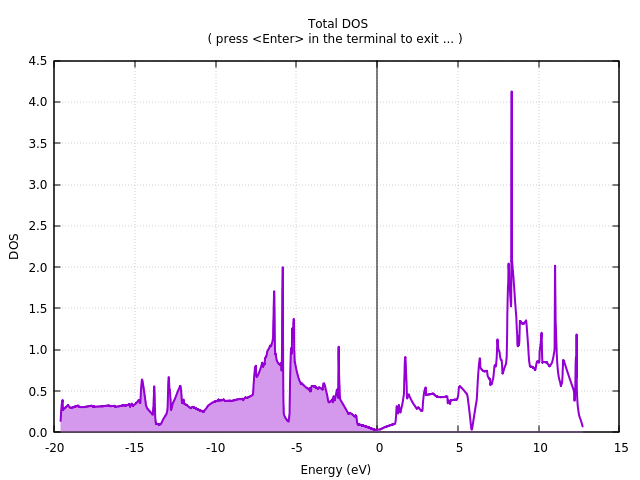
\includegraphics[scale = 0.6]{figs/D1/dos.png}
      \caption{DoS para la capa de grafeno: la zona sombreada representa ocupación electrónica, llegando hasta la energía de Fermi (línea negra).}
  \end{figure}

  Cuando hacemos el cálculo de las bandas, debemos pedir $calculation = 'bands'$ y con $nbnd$ especificamos el número de bandas: por default el programa sólo graficará las ocupadas, por lo que debemos poner un número mayor para observar bandas desocupadas. Otra diferencia es que le ponemos el camino de puntos K que queremos que siga.

  \begin{figure}[H]
      \centering
      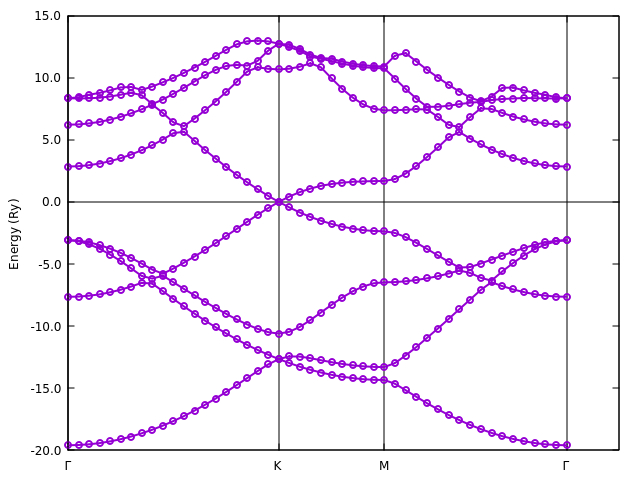
\includegraphics[scale = 0.6]{figs/D1/bandas.png}
      \caption{Estructura de bandas para el grafeno. Se observa el punto de Dirac al valor de la energía de Fermi.}
  \end{figure}

  Para seleccionar el camino de puntos k, podemos usar xcrysden. Para ello debemos ir a $Tools > k-path\ selection$ y esto nos permitirá seleccionar interactivamente el camino deseado.
